\documentclass[10pt]{article}
\usepackage{vmargin}
\setpapersize{A4}
\setmargins{2.5cm}% margen izquierdo
{.7cm}% margen superior
{16.5cm}% anchura del texto
{24.7cm}% altura del texto
{10pt}% altura de los encabezados
{1cm}% espacio entre el texto y los encabezados
{0pt}% altura del pie de página
{2cm}% espacio entre el texto y el pie de página
\usepackage{fancyhdr}%para encabezado
\usepackage{multicol}%hoja en columnas

\usepackage{graphicx} % figuras
\usepackage{subfigure} % subfiguras

\usepackage[spanish]{babel}
\usepackage[utf8]{inputenc}
\usepackage{comment}
\usepackage{multirow}

\begin{document}

\pagestyle{empty}
\thispagestyle{empty}
%\begin{flushright}
%\chead rLuis Miguel Pineda Daza \ \ \ 
%\end{flushright}


\begin{tabular}{c p{9cm} }
\multirow{2}{5cm}{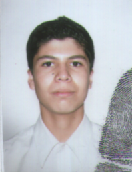
\includegraphics[scale=1]{foto_CV.png} }
&{\Large \textbf{Luis Miguel Pineda Daza}}

Licenciatura en Matem\'aticas Aplicadas y Computaci\'on 

Estudiante (octavo semestre)

\ 

{\large \textbf{Datos personales}}


\begin{tabular}{p{3cm} l}


\emph{Edad}&25 a\~nos\\

\emph{Tel\'efono} &55 25 01 77 41\\

\emph{E-mail}&
\textit{miguelpinedaza@gmail.com}\\

\emph{Direcci\'on}&Naucalpan, Estado de
Mex., CP 53270. \\



\end{tabular}
\end{tabular}
\\
\\
\\

\ 

\begin{large}
\textbf{Objetivos}
\end{large}


%Obtener un puesto de trainee de web aplicando mis conocimientos adquiridos y contribuir en el beneficio de la empresa.

%Obtener un puesto en el desarrollo de software aplicando mis conocimientos adquiridos y contribuir en el beneficio de la empresa.

%Obtener un puesto en el \'area de mantenimiento y soporte t\'ecnico aplicando mis conocimientos adquiridos y contribuir en el beneficio de la empresa.

%Obtener un puesto en el área de Auxiliar Contable aplicando mis conocimientos adquiridos y contribuir en el beneficio de la empresa.

%Obtener un puesto en el área de Actuario aplicando mis conocimientos adquiridos y contribuir en el beneficio de la empresa.

%Obtener un puesto en el área de Técnico en Electrónica aplicando mis conocimientos adquiridos y contribuir en el beneficio de la empresa.

%Obtener un puesto en el área de Asesor Telefónico aplicando mis conocimientos adquiridos y contribuir en el beneficio de la empresa.

%Obtener un puesto en el área de Atención con proveedores aplicando mis conocimientos adquiridos y contribuir en el beneficio de la empresa.

%Obtener un puesto en el área de Encargado de sucursal Comex aplicando mis conocimientos adquiridos y contribuir en el beneficio de la empresa.

%Obtener un puesto en el área de Bancked Developer aplicando mis conocimientos adquiridos y contribuir en el beneficio de la empresa.

%Obtener un puesto en el área de Customer Service aplicando mis conocimientos adquiridos y contribuir en el beneficio de la empresa.

Obtener un puesto en el área  especifica  aplicando mis conocimientos adquiridos y contribuir en el beneficio de la empresa.

\begin{comment}
Perfil del profesionista

El licenciado en Matemáticas Aplicadas y Computación es un profesionista capaz de utilizar las matemáticas y la computación de manera creativa para formular, analizar, diseñar, construir y automatizar soluciones a problemas reales. Durante su desempeño profesional ejercerá sus habilidades para actuar en equipos y adaptar métodos abstractos a la solución de problemas de orden práctico, así como a la modelación matemática y computacional de situaciones reales, con un pensamiento crítico, creativo e innovador de naturaleza inter y multidisciplinaria.

Estará capacitado para desempeñar actividades como:
Identificar problemas y proponer soluciones. Proponer constructos matemáticos-computacionales. Participar en equipos de investigación aplicada y documental en tecnologías de información, comunicación y desarrollo de software y hardware, para apoyar los procesos y servicios de una organización. Ofrecer consultoría en áreas físico-matemáticas y económico-administrativas, en inteligencia artificial, en tecnologías de la información, sistemas y programas de última generación. Atender las necesidades empresariales a través de la capacitación o actualización académicas. Desarrollar y manejar software: de sistema, de aplicación para resolver necesidades específicas de negocio, científico, empotrado, de línea de producto, así como aplicaciones de inteligencia artificial basadas en la Web y dispositivos móviles. Desempeñar la docencia en niveles de pregrado.
Objetivo

Desarrollar en el alumno la capacidad de aplicar creativamente las matemáticas y técnicas computacionales para analizar, evaluar y resolver problemas por medio de modelos en diversas áreas de conocimiento.
Características y habilidades recomendables del estudiante

El estudiante de Matemáticas Aplicadas y Computación debe poseer los conocimientos necesarios del área físico-matemática, contar con facilidad y razonamiento lógico, capacidad de concentración, de análisis y síntesis; tener una gran creatividad y curiosidad científica, así como de disciplina y constancia en el estudio y habilidad para el trabajo en equipo.
\end{comment}


\ 

%El esfuerzo de mi trabajo debe estar en proporci\'on a mi salario.







\begin{large}
\textbf{Educaci\'on}
\end{large}


Licenciatura en Matem\'aticas Aplicadas y Computaci\'on.  (octavo semestre).

Facultad de Estudios Superiores Acatl\'an

\ 

%Enfocado en la soluci\'on de problemas mediante modelos matem\'aticos y computaci\'on con el uso de las tecnolog\'ias emergentes, interactuando con diferentes \'areas del conocimiento y disciplinas.



\begin{large}
\textbf{Conocimiento}
\end{large}

Experiencia en la plataforma de eCommerce MAGENTO, realizando customizaciones de archvivos  css / xml / phtml / js y la creación de templates y layouts.


Manejo de lenguajes de programaci\'on: C, C++,  SQL, Python, Java, JavaScript, Html, PHP y CSS, y manejo de Office (excel avanzado). 


Realice mi servicio social en el Programa de Apoyo a Proyectos para la Innovaci\'on y Mejoramiento de la Ense\~nanza (PAPIME), realizando un Taller De Mantenimiento y Soporte T\'ecnico %con el tema de Instalaci\'on y Configuraci\'on de un Sistema Operativo 
con el Dr. Eduardo Eloy Loza Pacheco.


\ 

\begin{large}
\textbf{Experiencia laboral}
\end{large}

\ 

\textbf{doto.com.mx}  Desarrollador.

noviembre 2019 - febrero 2020

Mantenimiento de la pagina web doto.com.mx desarrollando backend y frontend.

\ 

\textbf{Promociones y Display Marketing.} Sistemas y Soporte.

agosto 2019 - septiembre 2019

Manejo de base de datos, plataforma y aplicación, altas de eventos, generar usuarios y contraseñas.

\ 

\textbf{McDonald's, Naucalapan, M\'ex.}
Empleado General
 

junio,2016 - agosto,2016 y junio,2017 - agosto,2017

Conocimiento en cocina y atenci\'on al cliente.

\ 

\textbf{Empacador de pan, MEGA San Mateo.}
Empleado general


noviembre,2016 - enero,2017

Elaboraci\'on del producto y atenci\'on al cliente

\ 

\textbf{Burger King M\'exico - Naucalpan, M\'ex. 
}L\'ider de producci\'on


 
febrero,2015 - septiembre,2015

Manejo de tiempos y temperaturas de la producci\'on del producto así como la evaluaci\'on de empleados.

\ 




\ 

\begin{large}
\textbf{Logros}
\end{large}


\ 

Diploma especial por reconocimiento a la labor de excelencia operativa en Burger King M\'exico.

\ 

Reconocimiento por haber impartido la ponencia ``La forma canónica local''  dentro del ``Seminario de Geometría Diferencial de Curvas y Superficies''  realizado en la Facultad de Estudios Superiores - Acatlán.



\end{document}